\documentclass[fleqn]{beamer}

\usepackage[british]{babel}
\usepackage{graphicx,ru,url}
\usepackage{amsmath}
% Use Times for math font and text font.
\RequirePackage[T1]{fontenc}
%\RequirePackage{txfonts}
% bold math must be loaded after Times font
\usepackage{bm}
\usepackage{booktabs} % nice rules (thick lines) for tables
\usepackage{microtype} % improves typography for PDF
\usepackage{xcolor} % Allows colors in fonts
\usepackage{tikz} % Allows creation of tikz pictures
\usepackage{verbatim}
\usetikzlibrary{arrows,shapes,snakes}
\usetikzlibrary{patterns}
\usepackage{url}
\usepackage{ifthen}

% The title of the presentation:
%  - first a short version which is visible at the bottom of each slide;
%  - second the full title shown on the title slide;
\title[Geant4 vs MCNP]{
    Geant4 Workshop}

% Optional: a subtitle to be displayed on the title slide
%\subtitle{Show where you're from}

% The author(s) of the presentation:
%  - again first a short version to be displayed at the bottom;
%  - next the full list of authors, which may include contact information;
\author[Wenkai Fu]{
    Wenkai Fu\\
    Prof. Jeremy A. Roberts}

% The institute:
%  - to start the name of the university as displayed on the top of each slide
%    this can be adjusted such that you can also create a Dutch version
%  - next the institute information as displayed on the title slide
\institute[Kansas State University]{
    Mechanical and Nuclear Engineering \\
    Kansas State University}

% Add a date and possibly the name of the event to the slides
%  - again first a short version to be shown at the bottom of each slide
%  - second the full date and event name for the title slide
\date[CORPS, 2/8/2019]{
    CORPS Workshop\\
    Feb. 8, 2019}

\begin{document}
    % These two commands allow bonus slides at the end
    % The bonus slides will not be numbered
    \newcommand{\beginbackup}{
        \newcounter{framenumbervorappendix}
        \setcounter{framenumbervorappendix}{\value{framenumber}}
    }
    \newcommand{\backupend}{
        \addtocounter{framenumbervorappendix}{-\value{framenumber}}
        \addtocounter{framenumber}{\value{framenumbervorappendix}}
    }
    
    \begin{frame}
        \titlepage
    \end{frame}
    
    \section{Section 1}
    
    \begin{frame}
        \frametitle{Overview of Geant4 and MCNP Inputs}
 \def\iwidth{4.5}
 \def\iheight{1.5}
 % distance between boxes in x or y axis is 1
 % origin at left lower conner of the detector construction box
 \centering
 \begin{tikzpicture}[scale=0.6, every node/.style={scale=0.6}]
  \draw  (0, 0) rectangle (\iwidth, \iheight) node at (\iwidth / 2, \iheight / 2) {detector construction};
  \draw (\iwidth + 1, 0) rectangle (\iwidth + 1 + \iwidth, \iheight) node at (\iwidth + 1 + \iwidth / 2, \iheight / 2) {physics list};
  \draw (\iwidth * 2 + 2, 0) rectangle (\iwidth * 3 + 2, \iheight) node at (\iwidth * 2 + 2 + \iwidth / 2, \iheight / 2) {action initialization};
  
  % connect lines between three initialization classes and the simulation box
%   \foreach \x in {0, 1, 2}
%   \draw ({\iwidth / 2 + \x * (\iwidth + 1)}, \iheight) -- ({\iwidth / 2 + \x * (\iwidth + 1)}, \iheight + 1);
%   \draw (\iwidth / 2, \iheight + 1) -- (\iwidth * 2.5 + 2, \iheight + 1);
%   \draw (\iwidth * 1.5 + 1, \iheight + 1) -- (\iwidth * 1.5 + 1, \iheight  + 2);
  
%   % simulation box
%   \draw (\iwidth + 1, \iheight + 2) rectangle (\iwidth * 2 + 1, \iheight * 2 + 2) node at (\iwidth * 1.5 + 1, \iheight * 1.5 + 2) {Geant4 simulation};
  
  % user actions
  \draw [<->, >= latex, double, thick] (\iwidth * 2 + 2 + \iwidth / 2, 0) -- (\iwidth * 2 + 2 + \iwidth / 2, -1);
  
  \foreach \y / \ilabel in {0/primary generator, 1/run action, 2/event action, 3/step action}{
  \draw (\iwidth * 2 + 2, {-1 - \y * (\iheight + 1)}) rectangle (\iwidth * 3 + 2, {-1 - \y * (\iheight + 1) - \iheight}) node at (\iwidth * 2 + 2 + \iwidth / 2, {-1 - \y * (\iheight + 1) - \iheight / 2}) {\ilabel};
  % plus sign
  \ifthenelse{\y<3} % seems there is an int operation, e.g., \y<3.8 = \y<3, which excludes \y=3
  {\node at (\iwidth * 2 + 2 + \iwidth / 2, {-1 - \iheight - 0.5 - \y * (\iheight + 1)}) {\textbf{+}};}
  
  % tally card
  % vertical connect lines
  \ifthenelse{\y>0}{\draw [dashed] (\iwidth * 2 + 2, {-1 - \y * (\iheight + 1) - \iheight / 2}) -- (\iwidth * 2 + 1.5, {-1 - \y * (\iheight + 1) - \iheight / 2});}
  }
  
  % tally card
  \draw [dashed] (\iwidth * 2 + 1.5, -2 - \iheight * 1.5) -- (\iwidth * 2 + 1.5, {-1 - 3 * (\iheight + 1) - \iheight / 2});
  \draw [dashed] (\iwidth * 2 + 1.5, -3 - \iheight * 2.5) -- (\iwidth * 2+1, -3 - \iheight * 2.5);
  \def\y{2}
  \draw [blue] (\iwidth + 1, {-1 - \y * (\iheight + 1)}) rectangle (\iwidth * 2 + 1, {-1 - \y * (\iheight + 1) - \iheight}) node [black] at (\iwidth + 1 + \iwidth / 2, {-1 - \y * (\iheight + 1) - \iheight / 2}) {tally card};
  
  % physics card
  \draw [blue] (\iwidth + 1, -1) rectangle (\iwidth * 2 + 1, -1 - \iheight) node [black] at (\iwidth + 1 + \iwidth / 2, -1 - \iheight / 2) {physics card};
  \draw [dashed] (\iwidth * 1.5 + 1, 0) -- (\iwidth * 1.5 + 1, -1);
  
  % source card
  \draw [blue] (\iwidth + 1, -2 - \iheight) rectangle (\iwidth * 2 + 1, -2 - \iheight * 2) node [black] at (\iwidth + 1 + \iwidth / 2, -2 - \iheight - \iheight / 2) {source card (sdef)};
  \draw [dashed] (\iwidth * 1.5 + 1, -2 - \iheight) -- (\iwidth * 1.5 + 1, -2 - \iheight + 0.5) -- (\iwidth * 2 + 1.5, -2 - \iheight + 0.5) -- (\iwidth * 2 + 1.5, -1 - \iheight / 2) -- (\iwidth * 2 + 2, -1 - \iheight / 2);
  
  % geometry and material cards
  \draw [dashed] (\iwidth / 2, 0) -- (\iwidth / 2, -1);
  \draw [blue] (0, -1) rectangle (\iwidth, -2 - \iheight * 2) node [align=left, black] at (\iwidth / 2, {(-3 - \iheight * 2)/2}) {surface card\\cell card\\material card};
 \end{tikzpicture}
    \end{frame}
    
    \begin{frame}
    \frametitle{Install Geant4 10.3}
    Geant4 10.3 requires cmake 3.3+ and GNU compiler 4.8.2+
    \begin{enumerate}
     \item Install Anaconda: \url{https://docs.anaconda.com/anaconda/install/linux/}\\
           \textcolor{blue}{conda install -c anaconda cmake}
     \item mkdir \$HOME/opt/geant4\_10\_3\_p03 $\Leftarrow$ build, src, install
     \item copy Geant4 source to src, set.cmake to build
     \item In build, \textcolor{blue}{cmake -C set.cmake ../src}, \textcolor{blue}{make -jN}, \textcolor{blue}{make install}
     \item copy data to \$HOME/opt/geant4\_10\_3\_p03/install/share/Geant4-10.3.3/
     \item add to .bashrc\\
           . \$HOME/opt/geant4\_10\_3\_p03/install/bin/geant4.sh\\
           \small export CMAKE\_PREFIX\_PATH=\$HOME/opt/geant4\_10\_3\_p03/install
    \end{enumerate}

    \end{frame}
    
    

    \begin{frame}
     \frametitle{Installation on Eigendoit}
     \begin{block}{MCNP}
      export DATAPATH=/share/apps/mcnp/MCNP\_DATA\\
      export PATH=\$PATH:/share/apps/mcnp/MCNP\_CODE/bin
     \end{block}

     \begin{block}{Geant4}
     \small
     export CMAKE\_PREFIX\_PATH=\\/home/wenkaifu/opt/geant4/geant4.10.03.p01/install\\
     . /home/wenkaifu/opt/geant4/geant4.10.03.p01/install/bin/geant4.sh\\
     \vspace{.2cm}
     alias cmake="/home/wenkaifu/opt/cmake/bin/cmake"\\
export CC=/home/wenkaifu/opt/gcc/install/bin/gcc\\
export CXX=/home/wenkaifu/opt/gcc/install/bin/g++\\
export LD\_LIBRARY\_PATH=\\/home/wenkaifu/opt/gcc/install/lib64:\$LD\_LIBRARY\_PATH

alias g++="/home/wenkaifu/opt/gcc/install/bin/g++"\\
alias gcc="/home/wenkaifu/opt/gcc/install/bin/gcc"
     \end{block}

    \end{frame}
    
%     \begin{frame}
%         \frametitle{MSND Geometry}
%         \begin{columns}[c]
%             \begin{column}{0.6\textwidth} % split the columns 50/50
%                 \centering
% \def\trench{1.6}
% \def\wall{1}
% \def\top{9.5}
% \def\bot{3}
% \def\pcontact{0.2}
% 
% \begin{tikzpicture}[scale=0.3, every node/.style={scale=0.7}]
% \draw (0, 0) rectangle (\wall + 6 * \trench + 6 * \wall, 10);
% % au contacts
% \draw [fill = black] (0, 0) rectangle (\wall + 6 * \trench + 6 * \wall, -0.3);
% \draw [fill = black] (0, \top + \pcontact) rectangle (\wall + \pcontact, 10);
% \draw [fill = black] (\wall * 7 + 6 * \trench, 10) rectangle (\wall * 7 + 6 * \trench - \wall - \pcontact, \top + \pcontact);
% 
% % n-type contact
% \draw [fill = black!10!white] (0.5, 0) rectangle (\wall + 6 * \trench + 6 * \wall - 0.5, 0.5);
% 
% \draw [pattern = north west lines] (0, \top) -- (\wall, \top) -- (\wall, \bot) -- (\trench + \wall, \bot) -- (\trench + \wall, \top) -- (\trench + 2*\wall, \top) -- (\trench + 2 * \wall, \bot) -- (2 * \trench + 2 * \wall, \bot) -- (2 * \trench + 2 * \wall, \top) -- (2 * \trench + 3 * \wall, \top) -- (2 * \trench + 3 * \wall, \bot) -- (3 * \trench + 3 * \wall, \bot) -- (3 * \trench + 3 * \wall, \top) -- (3 * \trench + 4 * \wall, \top) -- (3 * \trench + 4 * \wall, \bot) -- (4 * \trench + 4 * \wall, \bot) -- (4 * \trench + 4 * \wall, \top) -- (4 * \trench + 5 * \wall, \top) -- (4 * \trench + 5 * \wall, \bot) -- (5 * \trench + 5 * \wall, \bot) -- (5 * \trench + 5 * \wall, \top) -- (5 * \trench + 6 * \wall, \top) -- (5 * \trench + 6 * \wall, \bot) -- (6 * \trench + 6 * \wall, \bot) -- (6 * \trench + 6 * \wall, \top) -- (6 * \trench + 7 * \wall, \top) -- (6 * \trench + 7 * \wall, 10) -- (0, 10) -- (0, \top); 
% 
% % p-type contact
% \draw [fill = gray] (0, \top) -- (\wall, \top) -- (\wall, \bot) -- (\trench + \wall, \bot) -- (\trench + \wall, \top) -- (\trench + 2*\wall, \top) -- (\trench + 2 * \wall, \bot) -- (2 * \trench + 2 * \wall, \bot) -- (2 * \trench + 2 * \wall, \top) -- (2 * \trench + 3 * \wall, \top) -- (2 * \trench + 3 * \wall, \bot) -- (3 * \trench + 3 * \wall, \bot) -- (3 * \trench + 3 * \wall, \top) -- (3 * \trench + 4 * \wall, \top) -- (3 * \trench + 4 * \wall, \bot) -- (4 * \trench + 4 * \wall, \bot) -- (4 * \trench + 4 * \wall, \top) -- (4 * \trench + 5 * \wall, \top) -- (4 * \trench + 5 * \wall, \bot) -- (5 * \trench + 5 * \wall, \bot) -- (5 * \trench + 5 * \wall, \top) -- (5 * \trench + 6 * \wall, \top) -- (5 * \trench + 6 * \wall, \bot) -- (6 * \trench + 6 * \wall, \bot) -- (6 * \trench + 6 * \wall, \top) -- (6 * \trench + 7 * \wall, \top) -- 
% (6 * \trench + 7 * \wall, \top + \pcontact) -- (6 * \trench + 6 * \wall - \pcontact, \top + \pcontact) -- (6 * \trench + 6 * \wall - \pcontact, \bot + \pcontact) -- (6 * \wall + 5 * \trench + \pcontact, \bot + \pcontact) -- (6 * \wall + 5 * \trench + \pcontact, \top + \pcontact) -- (5 * \wall + 5 * \trench - \pcontact, \top + \pcontact) -- (5 * \wall + 5 * \trench - \pcontact, \bot + \pcontact) -- (5 * \wall + 4 * \trench + \pcontact, \bot + \pcontact) -- (5 * \wall + 4 * \trench + \pcontact, \top + \pcontact) -- (4 * \wall + 4 * \trench - \pcontact, \top + \pcontact) -- (4 * \wall + 4 * \trench - \pcontact, \bot + \pcontact) -- (4 * \wall + 3 * \trench + \pcontact, \bot + \pcontact) -- (4 * \wall + 3 * \trench + \pcontact, \top + \pcontact) -- (3 * \wall + 3 * \trench - \pcontact, \top + \pcontact) -- (3 * \wall + 3 * \trench - \pcontact, \bot + \pcontact) -- (3 * \wall + 2 * \trench + \pcontact, \bot + \pcontact) -- (3 * \wall + 2 * \trench + \pcontact, \top + \pcontact) -- (2 * \wall + 2 * \trench - \pcontact, \top + \pcontact) -- (2 * \wall + 2 * \trench - \pcontact, \bot + \pcontact) -- (2 * \wall + \trench + \pcontact, \bot + \pcontact) -- (2 * \wall + \trench + \pcontact, \top + \pcontact) -- (\wall + \trench - \pcontact, \top + \pcontact) -- (\wall + \trench - \pcontact, \bot + \pcontact) -- (\wall + \pcontact, \bot + \pcontact) -- (\wall + \pcontact, \top + \pcontact) -- (0, \top + \pcontact) -- (0, \top);
% 
% % label
% \draw [<-] (1, 0.25) -- (-1, 1) node [left, align = left] {n-type\\contact};
% \draw [<-] (\wall + 0.5 * \pcontact, \top -3) -- (-1, \top-1) node [left, align = left] {p-type\\contact};
% \draw [<-] (\wall + 0.5 * \trench, \top + 0.1) -- (\wall + 0.5 * \trench + 0.2, \top + 0.1 + 1) node [above, align=left] {neutron\\converter};
% \draw [<-] (\wall * 3 + 2.5 * \trench, \top - 1.5) -- (\wall * 3 + 2.5 * \trench + 0.5, \top + 0.1 + 1) node [above] {trench};
% \draw [<-] (\wall * 4.5 + 4 * \trench, \top - 1.5) -- (\wall * 4.5 + 4 * \trench + 0.5, \top + 1.1) node [above] {wall};
% \node at (\wall * 3.5 + 3 * \trench, 1.5) {n-type Si};
% \draw [<->] (\wall * 7 + \trench * 6 + 0.5, 10) -- (\wall * 7 + \trench * 6 + 0.5, \bot) node [midway, right, align=left] {etch\\depth};
% \draw [<-] (7 * \wall + 6 * \trench - 0.5 * \wall, 10) -- (7 * \wall + 6 * \trench - 0.5 * \wall - 0.5 * \trench, \top + 1.1) node [above] {Au contact};
% % length label
% \draw [<->] (0, -1.2) -- (\wall + 6 * \trench + 6 * \wall, -1.2) node [midway, fill = white] {length};
% % trench wall width label
% \draw [<->] (\wall, \bot-\pcontact) -- (2 * \wall + \trench, \bot-\pcontact) node [below, midway] {T + W};
% 
% % neutron
% \draw [fill = blue] (\wall * 4 + 3.5 * \trench, 0.5 * \top + 0.5 * \bot) circle [radius = 0.2];
% \draw [<-] (\wall * 4 + 3.5 * \trench, 0.5 * \top + 0.5 * \bot + 0.2) -- (\wall * 4 + 3.5 * \trench, \top + 1.1) node [above] {n};
% \draw [fill = red, red] (\wall * 3.5 + 3 * \trench, 0.8 * \top) circle [radius = 0.2];
% \draw [fill = red, red] (\wall * 4.5 + 4 * \trench, 0.53 * \top) circle [radius = 0.2];
% \draw [->, thick, red] (\wall * 4 + 3.5 * \trench, 0.5 * \top + 0.5 * \bot) -- (\wall * 3.5 + 3 * \trench, 0.8 * \top);
% \draw [->, thick, red, dashed] (\wall * 4 + 3.5 * \trench, 0.5 * \top + 0.5 * \bot) -- (\wall * 4.5 + 4 * \trench, 0.53 * \top);
% 
% % bulk Si
% \draw [dashed, teal, ultra thick] (0, 0) rectangle (\wall + 6 * \trench + 6 * \wall, \bot);
% \node [teal, right, align = center] at (\wall + 6 * \trench + 6 * \wall, \bot / 2) {bulk\\Si};
% 
% \end{tikzpicture}
%             \end{column}
%             
%             \begin{column}{0.4\textwidth} % Other half of the column split
%             
%             
%                 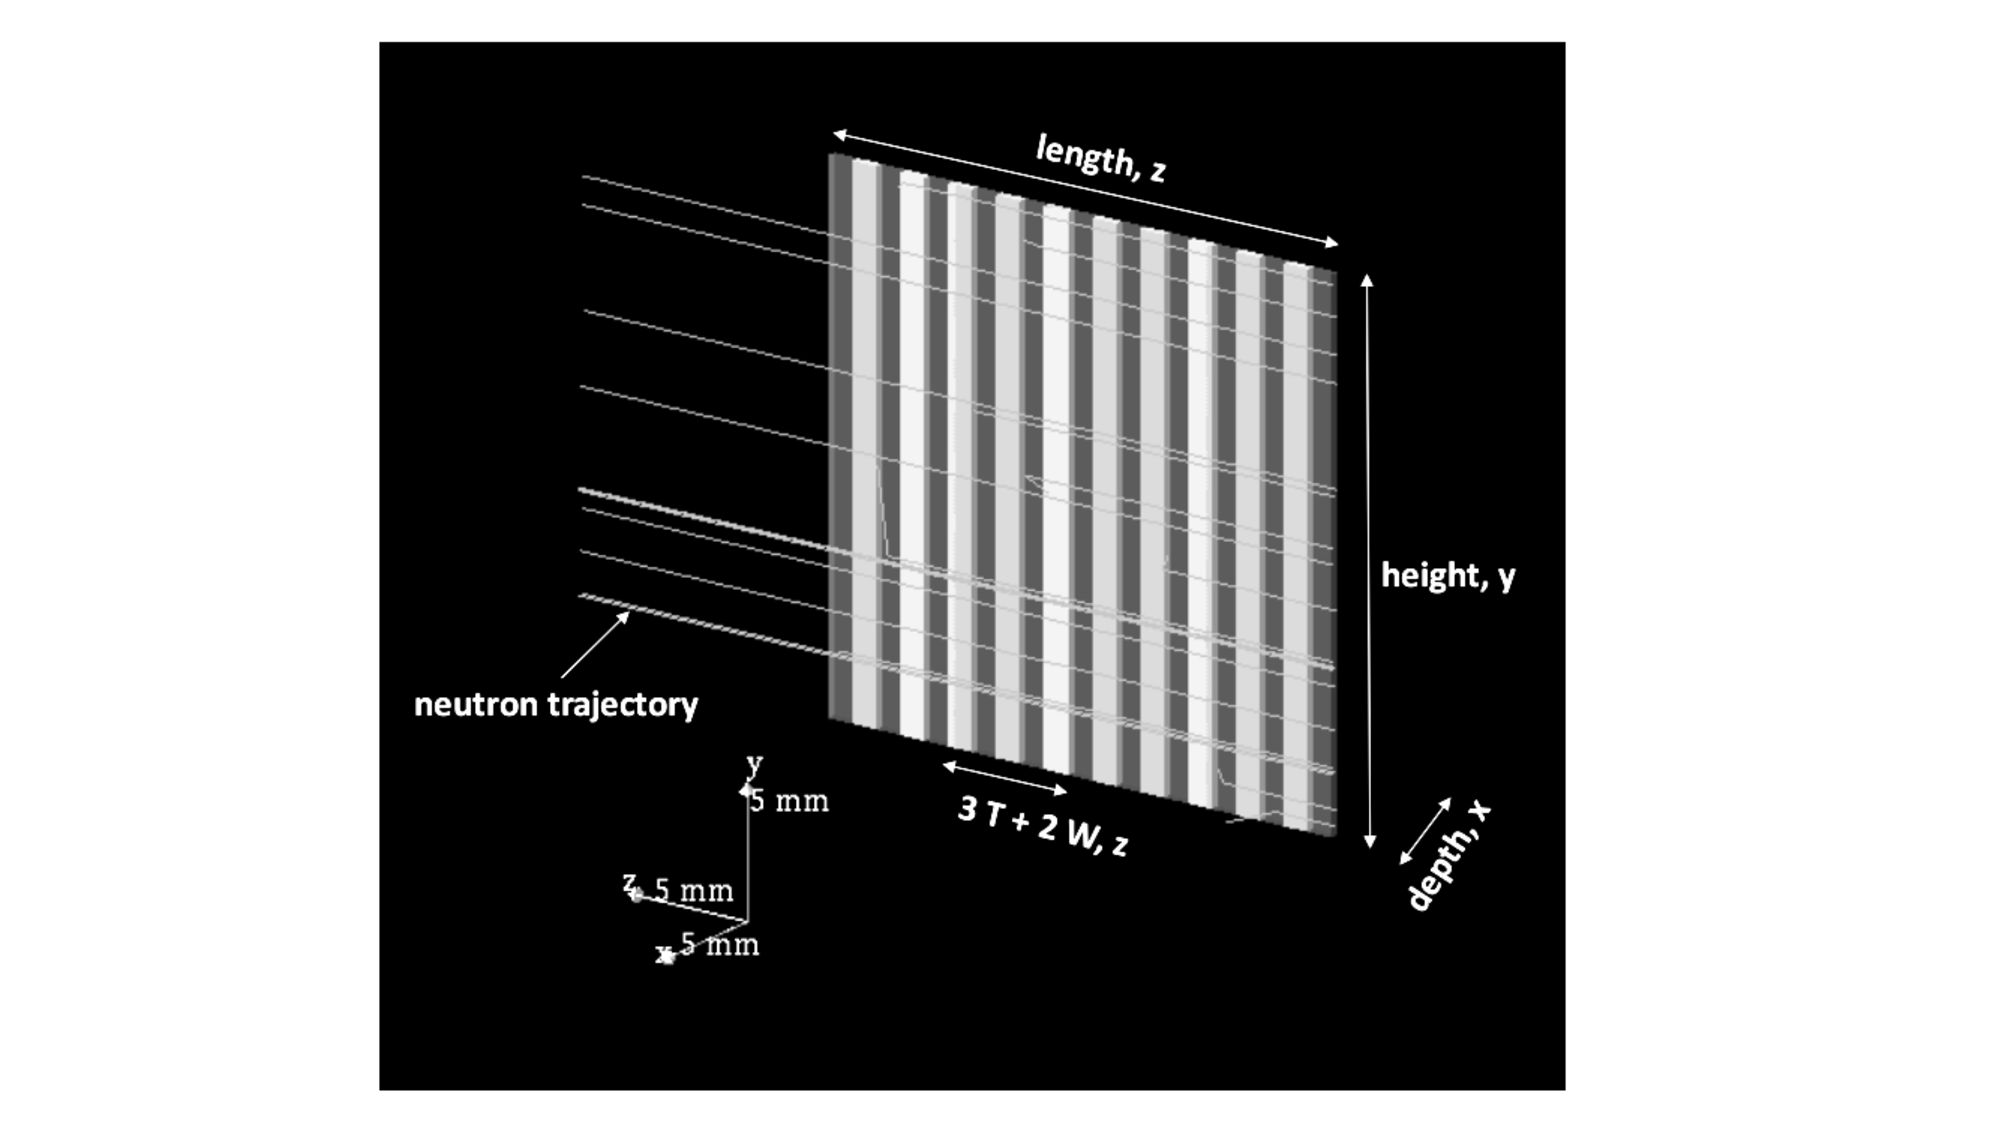
\includegraphics[trim={6cm 0 7cm 0}, clip, width = \textwidth]{./figures/msnd_g4gui_annotate_bw}
%                 
%                 
%             \end{column}
%         \end{columns}
%         \vspace{.8cm}
%         \centering
%         Height = 2~cm, Width = 350~$\mu$m
%     \end{frame}
    
    

    
   
    
%     \section{References}
%     
%     \begin{frame}[t,allowframebreaks]\label{lastframe}
%         \frametitle{References}
%         \bibliographystyle{ans}
%         % make a bibliography.bib file with your references in it
%         \bibliography{bibliography}
%     \end{frame}
    
\end{document}
